\section{First-Year Asteroid Observations}
\label{sec:samples}

\subsection{Known asteroids and repeated measurements}
\label{sec:known_population}

The primary sample contains \yrNAssoc\ associations to
\yrNKnown\ catalog identities on \yrNKnownNights\ observing
nights. Figure~\ref{fig:orbits} shows their orbital elements,
the number of observing nights, and the first-to-last measurement
span. Each identity contributes once to the orbital distribution,
while the sky map in Figure~\ref{fig:coverage} counts individual
measurements.

The main-belt region contains \yrNMainBelt\ identities,
or \yrMainBeltFrac\% of the sample. Other associations occupy
the inner-belt, Mars-crossing, outer-belt, Jupiter Trojan,
near-Earth, and distant-orbit regions. The near-Earth label
uses perihelion distance $q<1.3$~au, and the distant region
uses semimajor axis $a\geq5.4$~au. The Jupiter Trojan label
indicates the selected semimajor-axis region.

The distant region contains \yrNDistant\ positional-association
identities. The orbital distribution retains these sparse associations;
for such slowly moving sources, a positional coincidence alone need not
establish motion. Detailed local checks of selected earlier associations
are provided separately, rather than treating all distant-region points
as independently confirmed moving objects.

The median identity has \yrMedAssoc\ associations on
\yrMedNights\ nights, and the most frequently observed identity
appears on \yrMaxNights\ nights. The median first-to-last span
over all identities is \yrMedBaseline~days. The multi-night
distribution in Figure~\ref{fig:orbits}d shows the longer
baselines available for asteroid time series. Selecting objects
by measurement count, number of nights, and span provides samples
with different temporal coverage for subsequent work.

\begin{figure}[tbp]
\centering
\annualplot{fig07_orbits_and_revisits.pdf}{0.98\linewidth}
\caption{Known-asteroid associations during the first year, counted
once per catalog identity. (a,b) Catalog semimajor axis versus
eccentricity and inclination. Colors and symbols mark the adopted
orbital regions; the dashed curve is $q=1.3$~au. The Jupiter Trojan
region is selected by semimajor axis. Distant-region points include
all positional associations and are interpreted with the local
motion checks described in the text. (c) Number of observing
nights per identity. (d) First-to-last measurement span for the
multi-night subset. The semimajor-axis scales in (a,b) and the
count scales in (c,d) are logarithmic.}
\label{fig:orbits}
\end{figure}

The detection-weighted median solar elongation is
$\yrElongation^\circ$, with a minimum of
$\yrElongationMin^\circ$. Adjacent measurements of the same
identity within a night have a median measured angular rate
of \yrMeasuredRate~\rateunit. Appendix~\ref{app:geometry}
defines these quantities and shows their distributions.
Known-object association uses predicted positions directly,
so its angular-rate coverage extends beyond the interval
of the independent motion search.

\subsection{Single-night moving-source candidates}
\label{sec:candidates}

Restricting archived independent-search links to the science exposures
yields \yrNAuto\ automatic links
over \yrNSearchNights\ nights. Records with explicit image-review or completion evidence cover
\yrNReviewed\ links from \yrNReviewNights\ nights and retain
\yrNCandidates\ candidates containing \yrNCandidateMeasurements\
measurements on \yrNCandidateNights\ nights
(Table~\ref{tab:candidates}). A further 2,286 links from
25 nights have no explicit review-completion evidence and are listed
separately; they are not classified as rejected. The retained count
combines the previously audited subset with 56 additional positive
image-review records that satisfy the same exposure selection and excludes
subsequent explicit false-positive decisions. Each retained link contains
measurements in at least three distinct exposures within one
observing night. These links describe observed single-night
trajectories. Connections across nights and comparison with
orbital predictions establish their individual identities.

\begin{table}[tbp]
\centering
\caption{Single-Night Moving-Source Sample}
\label{tab:candidates}
\begin{tabular}{lr}
\toprule
Quantity & Number\\
\midrule
Automatic links & \yrNAuto\\
Links inspected in images & \yrNReviewed\\
Retained candidates & \yrNCandidates\\
Measurements in retained candidates & \yrNCandidateMeasurements\\
Links associated with C/2025~Y1 & \yrNCometLinks\\
Retained links without an established identity & \yrNUnidentified\\
\bottomrule
\end{tabular}
\tablecomments{Counts refer to links and their constituent
measurements. The automatic and image-inspected samples have
the observing coverage given in the text. The retained sample is the
reviewed subset, and the full-year review is not yet complete.}
\end{table}

Figure~\ref{fig:candidate} shows an example from 2026 February~10.
Its three exposure midpoints span approximately 79~min, and the
measured linear sky-plane rate is 61.34~\rateunit. The successive
positions illustrate the motion evidence supporting an individual
link. The spans and short-arc fit residuals of the retained
reviewed subset from the first year are compared in Appendix~\ref{app:shortarc}.

\begin{figure}[tbp]
\centering
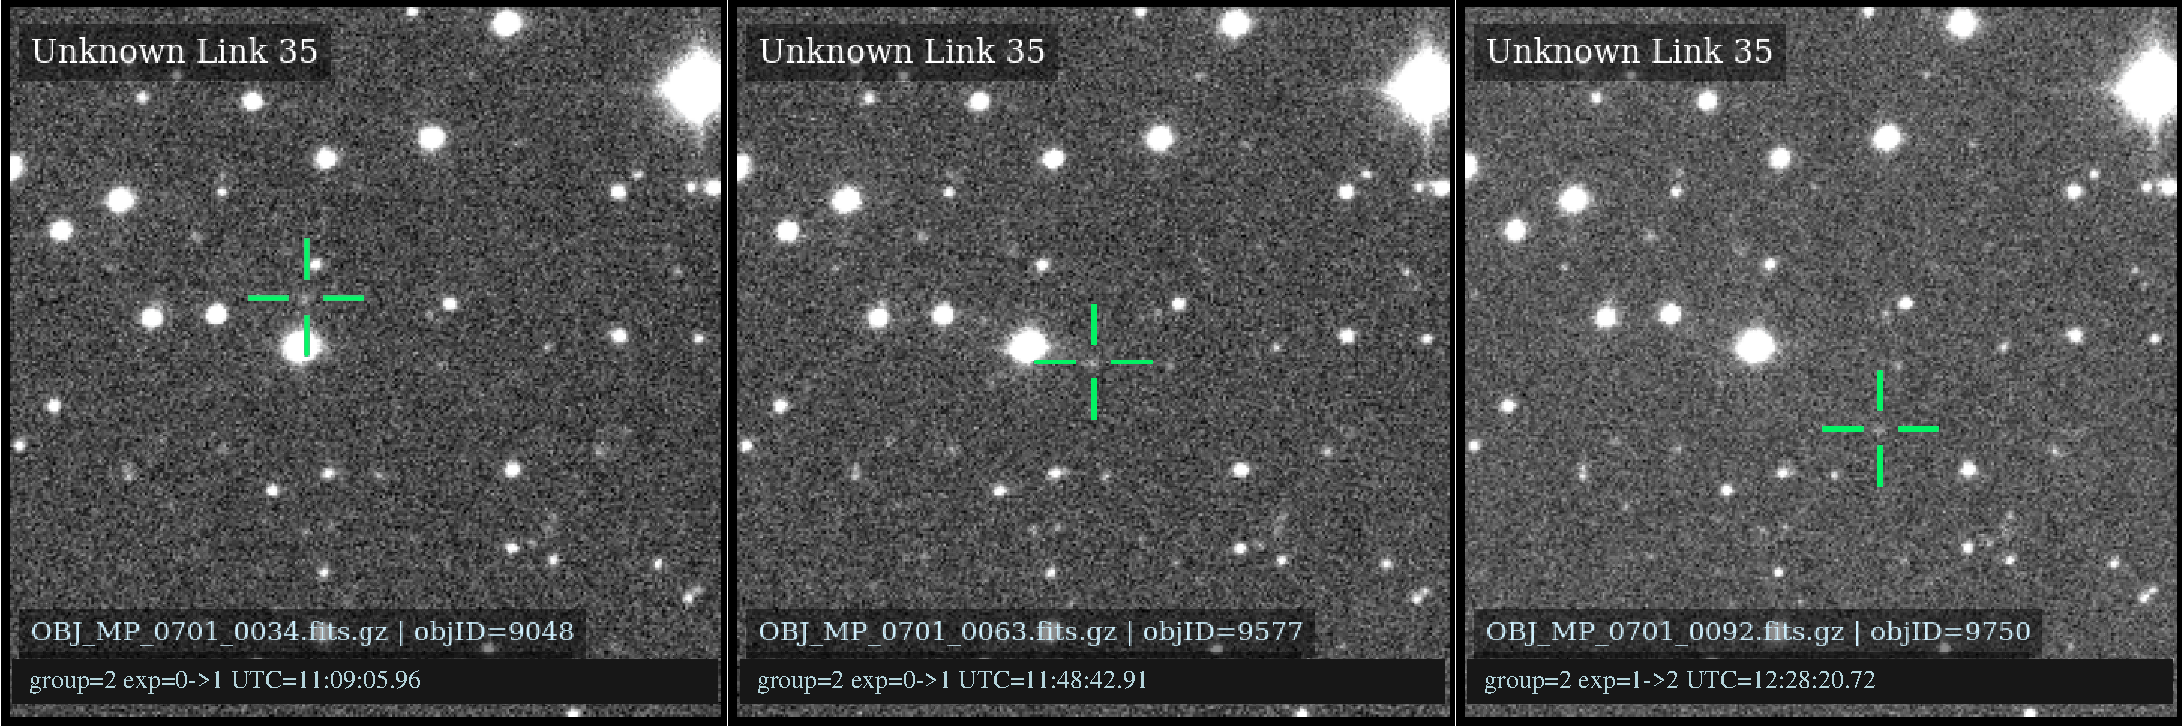
\includegraphics[width=\linewidth]{fig08_candidate.pdf}
\caption{Three images of the 2026 February~10 single-night
linkage 35, identified as \texttt{00000P2}. From left to right,
the UTC exposure midpoints are 11:09:05.96, 11:48:42.91,
and 12:28:20.72. The green marks locate the detections.
The fitted linear rate is approximately 61.34~\rateunit.}
\label{fig:candidate}
\end{figure}

Comparison with comet ephemerides associates \yrNCometLinks\
of the retained links with C/2025~Y1 (ATLAS). The comet remains
in the moving-source sample because the attribution catalog
contains asteroid orbits. For the \yrNUnidentified\ retained
links without established identities, the observations supply
positions, brightnesses, and apparent motion over the measured
arcs. Additional observations and cross-night association can
extend those arcs and determine how many objects they represent.
